\documentclass[aspectratio=169]{beamer}
\usepackage[utf8]{inputenc}
%\usepackage[authordate,backend=biber,natbib]{biblatex-chicago}
%\usepackage{booktabs}
%\addbibresource{growthreferences.bib}

%\usepackage{utopia} %font utopia imported

\usetheme{Madrid}
\usecolortheme{beaver}

%------------------------------------------------------------
%This block of code defines the information to appear in the
%Title page
\title[Mayer (1984)] %optional
{Endogenous Tariff Formation}

\subtitle{Wolfgang Mayer, \emph{American Economic Review}, 1984}

\author [Hauk] % (optional)
{William~R.~Hauk,~Jr.} %\inst{1} %\and J.~Doe\inst{2}} 

\institute[UofSC] % (optional)
{
  %\inst{1}%
  Darla Moore School of Business\\
  University of South Carolina
  %\and
  %\inst{2}%
  %Faculty of Chemistry\\
  %Very Famous University
}

\date[ECON 860, Fall 2021] % (optional)
{ECON 860 -- International Trade Theory\\Fall 2021}

\logo{
\includegraphics[height=1cm]{UofSC_Monogram_Stack_CMYK_G.jpg}}

%End of title page configuration block

%---------------------------------------------------------

\AtBeginSection[]
{
  \begin{frame}
    \frametitle{Table of Contents}
    \tableofcontents[currentsection]
  \end{frame}
}

%------------------------------------------------------------

\begin{document}

%The next statement creates the title page.
\frame{\titlepage}

%-------------------------------------------------------------

\section{Introduction}

%-------------------------------------------------------------

\begin{frame}{Trade and Distribution}

\begin{itemize}
    \item<1-> As noted previously, most of the time, international trade maximizes a country’s overall welfare, but has distributional effects within it.
    \item<2-> Distributional effects will create a demand for trade protection by some political constituency.
    \item<3-> Two ways that we can approach this.  First one is this paper by Mayer, who looks at determinants of the preferences of a median vote in society.  Economics is largely Heckscher-Ohlin.
    \item<4-> The other way is to look at protection as the outcome of competition between organized interest groups.  This is the approach of Grossman and Helpman (1994).  The economics is largely specific-factors based.
\end{itemize}
    
\end{frame}

%-------------------------------------------------------------

\begin{frame}{Previous Literature}

\begin{itemize}
    \item<1->  Early models in this area were done by Baldwin (1976, 1982), Brock and Magee (1978, 1980), and Findlay and Wellisz (1982).  ``Underlying premise of these studies is that political decisions on tariff rates are reflections of the selfish economic interests of voters, lobbying groups, politicians, or other decision makers in trade policy matters.”
    \item<2->  Baldwin in particular notes that, for a small country, zero tariffs are optimal if consumer preferences are homothetic, voters have perfect information, and income redistributions are costless.  If you relax any of these assumptions, tariff rates might be affected by politically powerful interest groups who stand to lose a lot from trade.
\end{itemize}
    
\end{frame}

%-------------------------------------------------------------

\begin{frame}{Mayer Contributions}
    
\begin{itemize}
    \item<1-> Mayer paper attempts to link the variation in tariff rates to factor-ownership distribution, voter eligibility, and participation rules.
    \item<2-> Unlike previous papers (e.g. Baldwin), voters are allowed to own more than one factor of production, although their shares will vary across voters.
    \item<3-> If there is majority voting with and no voting costs, the ``optimal” tariff will generally be determined by the median voter’s factor ownership profile.
    \item<4-> First take at the model uses a two-by-two Heckscher-Ohlin setup.  Second take uses a specific-factors multisector model.  Paper also looks at the configuration of factor-ownership distributions and voting rules that would result in free-trade.
\end{itemize}

\end{frame}

%-------------------------------------------------------------

\section{Optimal Tariff Rates in a Heckscher-Ohlin Model}

\subsection{Assumptions}

%-------------------------------------------------------------

\begin{frame}{Optimal Tariff Rates in a Heckscher-Ohlin Model – Assumptions}

\begin{itemize}
    \item<1-> Small open economy in which capital and labor are employed to produce two commodities, $ X_{1} $ and  $ X_{2} $.  Each resident of the country possesses one unit of labor ($ L_{i} =  1 $) and some non-negative amount of capital ($ K_{i} \ge 0 $).
    \item<2-> Other Heckscher-Ohlin assumptions apply – factors are mobile across industries, markets are competitive, constant returns to scale.  Preferences of a country’s inhabitants are assumed to be homothetic and identical, so that a redistribution of income does not affect aggregate demand if income remains constant.
\end{itemize}
    
\end{frame}

%-------------------------------------------------------------

\begin{frame}{Preferences}

\begin{itemize}
    \item<1-> Individual $ i $'s preferences are expressed by the indirect utility function:
    \begin{equation}
        U^{i}\left( p, y^{i} \right) \text{ where } i = 1,...,I
        \label{eq:utility1}
    \end{equation}
    where $ p $ is the relative price of good $ 1 $ in terms of good $ 2 $, and income $ y^{i} $ is measured in terms of good $ 2 $.
    \item<2-> There are three potential sources of income: wages, rents from capital, and redistributed tariff revenues:
    \begin{equation}
        y^{i} = w + rK^{i} + T^{i}
        \label{eq:income1}
    \end{equation}
\end{itemize}
    
\end{frame}

%-------------------------------------------------------------

\begin{frame}{Factor Ownership}

\begin{itemize}
    \item<1-> Mayer assumes that tariff revenue is redistributed in proportion to income from factor ownership, that is:
    \begin{equation}
        T^{i} = \phi^{i} T
        \label{eq:tariffi}
    \end{equation}
    where $ T $ is total tariff revenue and
    \begin{equation}
        \phi^{i} = \frac{w + rK^{i}}{wL + rK}
        \label{eq:phii}
    \end{equation}
    \item<2-> Substituting (\ref{eq:tariffi}) and (\ref{eq:phii}) into (\ref{eq:income1}) gives us:
    \begin{equation}
        y^{i} = \phi^{i}\left( wL + rK + T \right) = \phi^{i} Y
        \label{eq:income2}
    \end{equation}
    where $ Y $ is the economy's total income in terms of the second good.
\end{itemize}
    
\end{frame}

%-------------------------------------------------------------

\begin{frame}{Tariff Revenue}

Without loss of generality, we assume that for relevant tariff rates, the country incompletely specializes in the production of good $ 2 $ and imports good $ 1 $.  Total tariff revenues are expressed as:
\begin{equation*}
    T = t \pi M
\end{equation*}
where $ t $ is the tariff rate, $ \pi $ is the world price, and $ M $ is the quantity imported of good $ 1 $.
    
\end{frame}

%-------------------------------------------------------------

\subsection{Optimal Tariff Rates for Individuals}

%-------------------------------------------------------------

\begin{frame}{Optimal Tariff Rates for Individuals}

\begin{itemize}
    \item<1-> Because factor ownership differs among a country’s people, their welfare is not uniformly affected by a tariff increase.  Substituting (\ref{eq:income2}) into (\ref{eq:utility1}) gives us:
    \begin{equation}
        U^{i} = U^{i}\left( p, \phi^{i} Y \right)
        \label{eq:utility2}
    \end{equation}
    \item<2-> Let $ p = \pi \left( 1 + t \right) $ and differentiate (\ref{eq:utility2}) with respect to $ t $:
    \begin{equation}
        \frac{\partial U^{i}}{\partial t} = \frac{\partial U^{i}}{\partial y^{i}} \times \left[ -\phi^{i} \pi D_{1} + \phi^{i} \frac{\partial Y}{\partial t} + Y \frac{\partial \phi^{i}}{\partial t} \right]
        \label{eq:dUdt1}
    \end{equation}
    where $ D_{1} $ is the aggregate demand for good $ 1 $ (derived from Roy’s identity / envelope theorem).
\end{itemize}
    
\end{frame}

%-------------------------------------------------------------

\begin{frame}{Aggregate Income}

\begin{itemize}
    \item<1-> The economy’s aggregate income is given by:
    \begin{equation}
        Y = wL + rK + T = pX_{1} + X_{2} + t \pi M
        \label{eq:aggincome}
    \end{equation}
    \item<2-> If we differentiate (\ref{eq:aggincome}) by $ t $, we get:
    \begin{equation}
        \frac{\partial Y}{\partial t} = \pi D_{1} + t \pi \frac{\partial M}{\partial t}
        \label{eq:dYdt}
    \end{equation}
    where $ \frac{\partial M}{\partial t} < 0 $.
\end{itemize}
    
\end{frame}

%-------------------------------------------------------------

\begin{frame}{Tariffs and Welfare}

\begin{itemize}
    \item<1-> Substituting (\ref{eq:dYdt}) back into (\ref{eq:dUdt1}) gets us:
    \begin{equation}
        \frac{\partial U^{i}}{\partial t} = \frac{\partial U^{i}}{\partial y^{i}} \times \left[ \phi^{i} t \pi \frac{\partial M}{\partial t} + Y \frac{\partial \phi^{i}}{\partial t} \right]
        \label{eq:dUdt2}
    \end{equation}
    \item<2->There are two channels through which a tariff will affect individual welfare – the fall in tariff-weighted imports ( $ \phi^{i} t \pi \frac{\partial M}{\partial t} $), which is always negative, and the change in person $ i $'s income share ($ Y \frac{\partial \phi^{i}}{\partial t} $), which could be either positive or negative depending on that's person's factor endowment.
\end{itemize}
    
\end{frame}

%-------------------------------------------------------------

\begin{frame}{``Optimal" Tariffs}

\begin{itemize}
    \item<1-> We can calculate person $ i $’s optimal tariff by setting $ \frac{\partial U^{i}}{\partial t} = 0 $:
    \begin{equation}
        t^{i^{*}} = - \left[ \frac{Y}{\frac{\partial M}{\partial t}} \right] \left[ \frac{\frac{\partial \phi^{i}}{\partial t}}{\phi^{i}} \right]
        \label{eq:optimalti}
    \end{equation}
    \item<2-> $ \frac{\partial M}{\partial t} < 0 $, so the optimal tariff is positive if $ \frac{\partial \phi^{i}}{\partial t} > 0 $ (the tariff increases the person's income share), zero if $ \frac{\partial \phi^{i}}{\partial t} = 0 $, and negative if $ \frac{\partial \phi^{i}}{\partial t} < 0 $.
\end{itemize}
    
\end{frame}

%-------------------------------------------------------------

\begin{frame}{Tariffs and Factor Ownership}

\begin{itemize}
    \item<1-> Relationship between a tariff and a person’s income depends on factor endowments, parameterized by $ \phi^{i} $.
    \item<2-> If we differentiate equation (\ref{eq:phii}) with respect to the tariff and apply the Heckscher-Ohlin model, we get:
    \begin{equation}
        \frac{\partial \phi^{i}}{\partial t} = \left[ \frac{wL}{\left( wL + rK \right)^{2} \left( 1 + t \right)} \right] \times \left[ \frac{r\left( k - k^{i} \right) \left( \hat{w} - \hat{r} \right)}{\hat{p}} \right]
        \label{eq:dphidt}
    \end{equation}
    where $ k = K / L $ and $ k^{i} = K^{i} / L $.
    \item<3-> The first term in brackets is positive.  From the Stolper-Samuelson theorem, we know that $ \frac{\left( \hat{w} - \hat{r} \right)}{\hat{p}} > 0 $ if the imported good is labor-intensive (and conversely if it is capital-intensive).
\end{itemize}
    
\end{frame}

%-------------------------------------------------------------

\begin{frame}{Endowment Levels}

\begin{itemize}
    \item<1-> Equation (\ref{eq:dphidt}) tells us that a person’s income share will be affected depending on their relative endowment of capital.
    \item<2-> If $ k > k^{i} $ (that is, person $ i $ has less than an average amount of capital), then a tariff on a labor intensive good will raise $ \phi^{i} $.
    \item<3-> If $ k < k^{i} $ (that is, person $ i $ has more than an average amount of capital), then a tariff on a labor intensive good will lower $ \phi^{i} $.
    \item<4-> The converse happens if the tariff is imposed on a capital-intensive good.
\end{itemize}
    
\end{frame}

%-------------------------------------------------------------

\begin{frame}{Optimal Tariff Rates in Summary}

Three conclusions can be drawn about individually optimal tariff rates:

\begin{enumerate}
    \item<1-> The optimal import tariff is positive (negative) for people who are relatively well (poorly) endowed with the import good’s intensively used factor.
    \item<2-> The greater the difference between individual and national endowment ratios, the greater the deviation of individually optimal tariff or subsidy rates from a free-trade policy.
    \item<3-> The optimal tariff rate is zero for each person whose personal capital-labor ownership ratio equals the national capital-labor endowment ratio.
\end{enumerate}
    
\end{frame}

%-------------------------------------------------------------

\section{Tariff Determination Under Majority Voting}

\subsection{Real Income Effects of Tariff Changes}

%-------------------------------------------------------------

\begin{frame}{Real Income Effects of Tariff Changes}

\begin{itemize}
    \item<1-> In order to understand how different voting rules affect tariffs, we must first look more closely at the real income effects of tariff changes.
    \item<2-> Measured in terms of good $ 2 $, the real income change of individual $ i $ resulting from the tariff increase is:
    \begin{equation*}
        B^{i}\left( k^{i}, t \right) = \frac{\partial U^{i}}{\partial t} / \frac{\partial U^{i}}{\partial y^{i}}
    \end{equation*}
    intuitively, how much the price of the good is changed by the tariff relative to how much income is changed by the tariff.
    \item<3-> $ \frac{\partial B^{i}}{\partial k^{i}} > 0 $ if the imported good is capital intensive, and conversely if it is labor-intensive.
\end{itemize} 
    
\end{frame}

%-------------------------------------------------------------

\begin{frame}{Capital Endowment and Preferred Tariffs}

\begin{itemize}
    \item<1-> To show that $ \frac{\partial B^{i}}{\partial k^{i}} > 0 $ for a capital intensive good, first find an individual $ j $ such that their capital endowment $ k^{j} $ would make the prevailing tariff rate would be optimal.
    \item<2-> That is, from equations (\ref{eq:optimalti}) and (\ref{eq:dphidt}):
    \begin{equation}
        t = -\left[ \frac{\gamma}{\pi\frac{\partial m}{\partial t}} \right] \left[ \frac{wL \left( \hat{w} - \hat{r} \right)}{\left( wL + rK \right) \hat{p} \left( 1 + t \right)}  \right] \left[ \frac{r \left( k - k^{j} \right)}{w + rk^{j}} \right]
        \label{eq:tforkj}
    \end{equation}
\end{itemize}
    
\end{frame}

%-------------------------------------------------------------

\begin{frame}{Deriving $ B^{i} $}

\begin{itemize}
    \item<1-> Using equation (\ref{eq:dUdt1}) we can rewrite $ B^{i} $ as:
    \begin{equation*}
        B^{i}\left( k^{i}, t \right) = \phi^{i} \left[ t \pi \frac{\partial M}{\partial t} +  Y \frac{\partial \phi^{i}}{\partial t} / \phi^{i} \right]
    \end{equation*}
    \item<2-> Substituting (\ref{eq:tforkj}) for $ t $ and (\ref{eq:dphidt}) for $ \frac{\partial \phi^{i}}{\partial t} $, $ B^{i} $ becomes:
    \begin{equation}
        B^{i} = -\left[ \frac{\hat{w} - \hat{r}}{\hat{p}\left( 1 + t \right)} \right] \left[ \frac{Ywr}{\left( w + r\tilde{k}^{j} \right) \left( wL + rK \right)} \right]\left[ k^{i} - \tilde{k}^{j} \right]
        \label{eq:Birevised}
    \end{equation}
    where $ -\frac{\hat{w} - \hat{r}}{\hat{p}} > 0 $ for a capital-intensive import good.
\end{itemize}
    
\end{frame}

%-------------------------------------------------------------

\begin{frame}{$ B^{i} $ and Capital Endowment}

\begin{itemize}
    \item<1-> Equation (\ref{eq:Birevised}) tells us that a given tariff raises (lowers) the $ i $th person’s real income if the $ i $th person’s capital-labor ratio exceeds (falls short of) the capital-labor endowment ratio $ \tilde{k}^{j} $ of the person for whom the tariff is optimal.
    \item<2-> Note that $ \frac{\partial B^{i}}{\partial k^{i}} > 0 $ if the first term is negative (the import good is capital-intensive).
\end{itemize}
    
\end{frame}

%-------------------------------------------------------------

\begin{frame}{Figure 1}

\begin{figure}
    \centering
    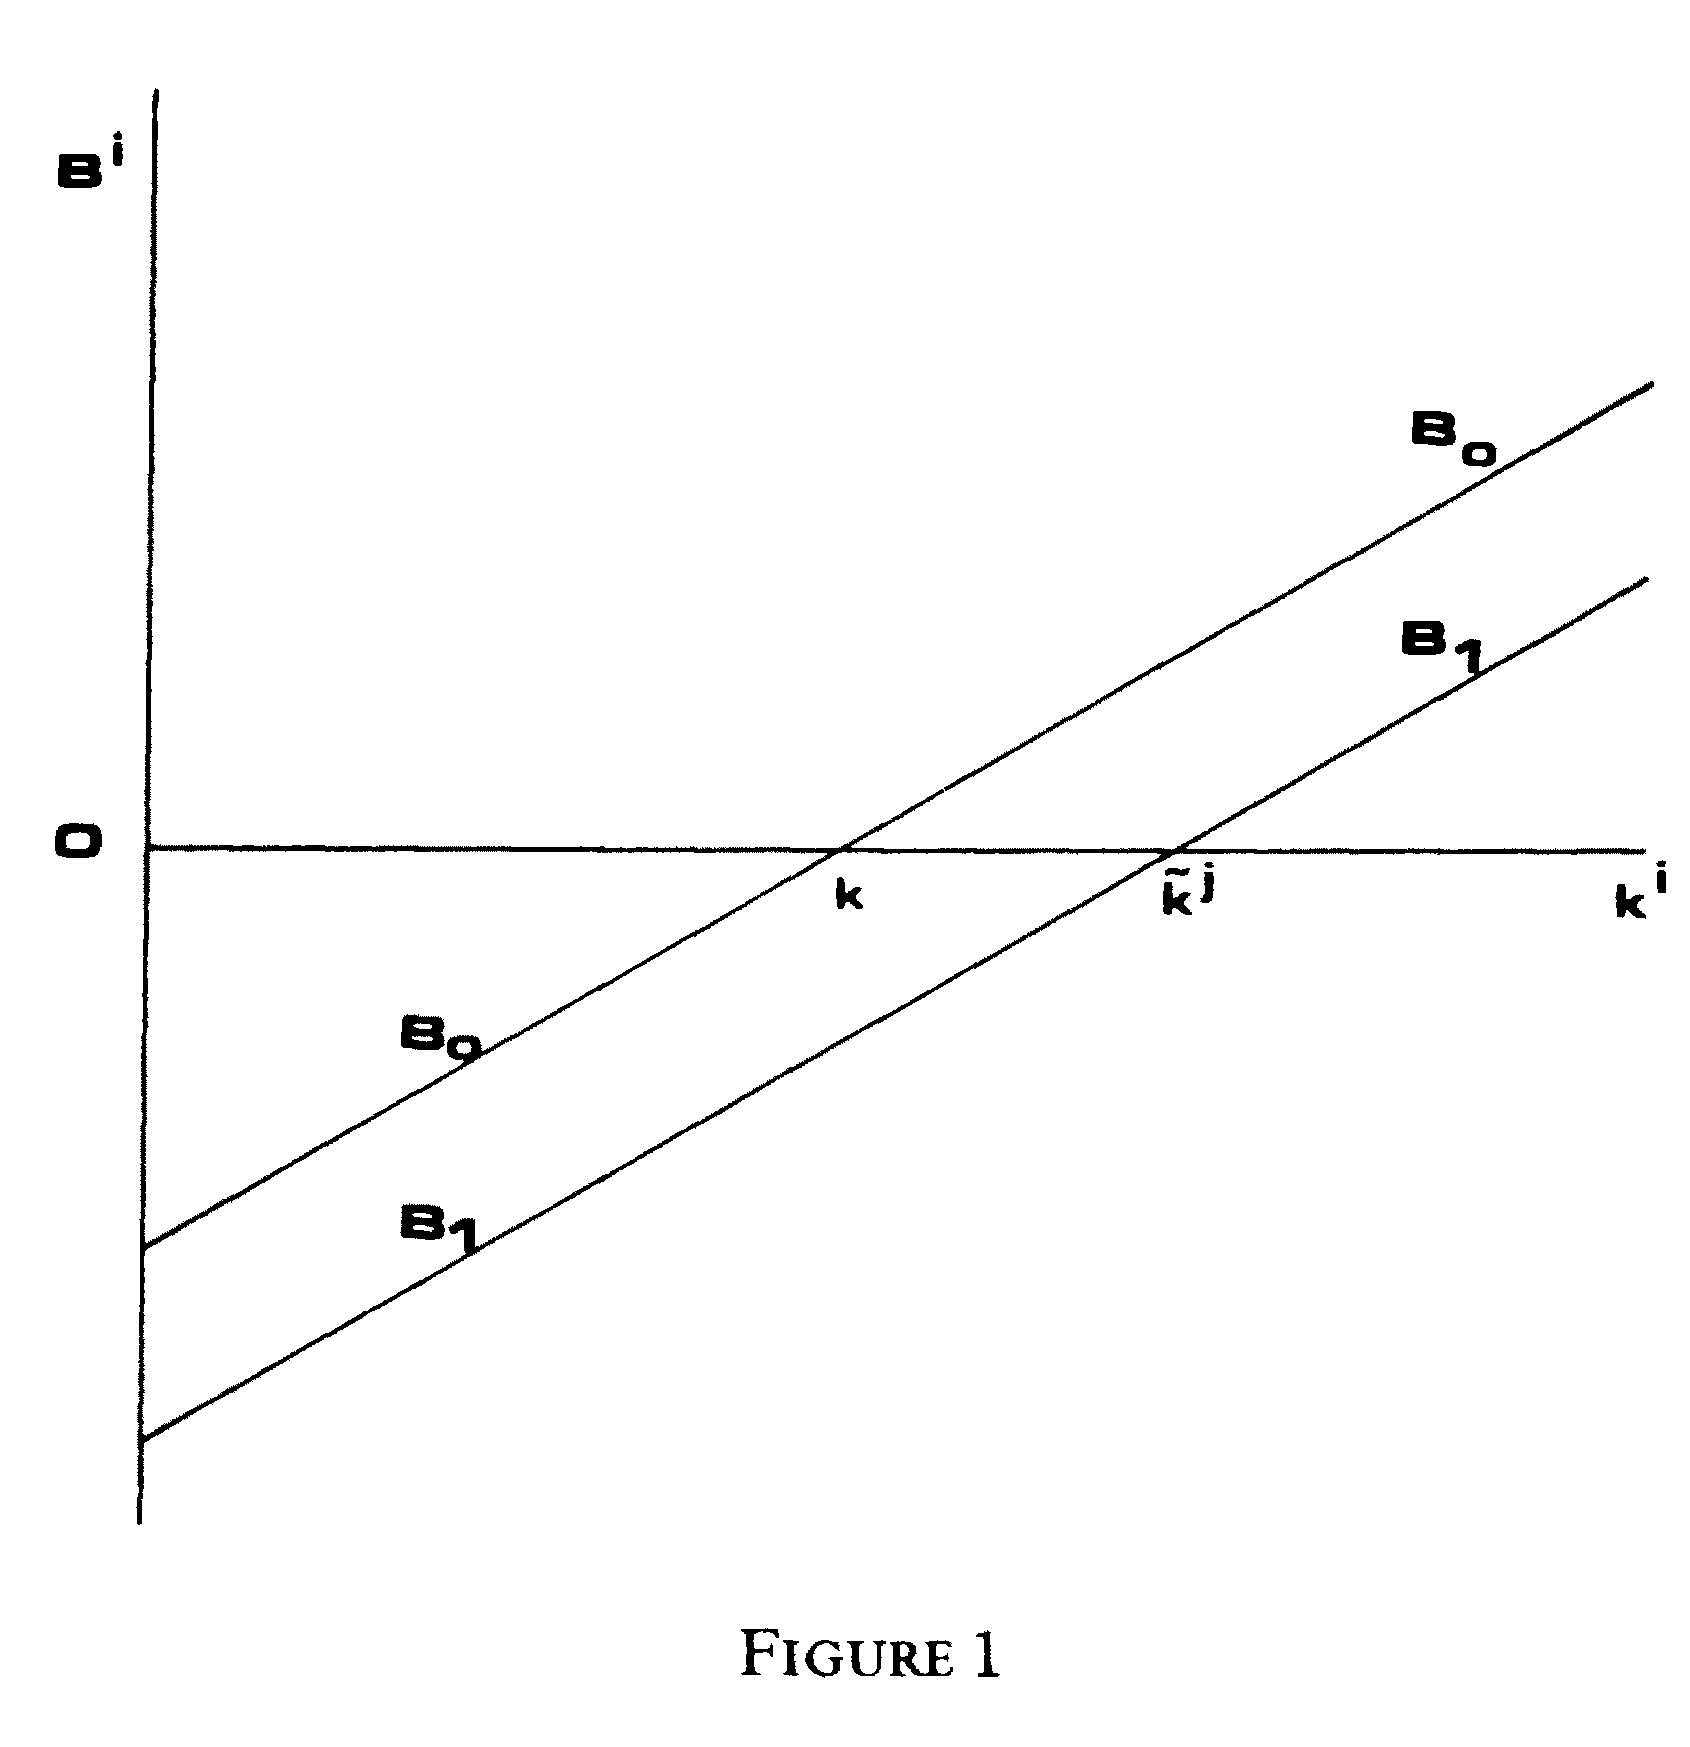
\includegraphics[scale=0.95]{MayerFig1.jpg}
    \label{fig:Fig1}
\end{figure}
    
\end{frame}

%-------------------------------------------------------------

\begin{frame}{Figure 1 and Preferences}

\begin{itemize}
    \item<1-> Figure 1 depicts an economy whose import competing industry is capital-intensive.
    \item<2-> Line $ B_{0} B_{0} $ represents the change in welfare from a tariff at free trade.
    \item<3-> $ B_{1} B_{1} $ represents the same for a positive tariff $ t $ for whom it is person $ j $’s optimal tariff. 
\end{itemize}
    
\end{frame}

%-------------------------------------------------------------

\subsection{Majority Voting Without Restrictions}

%-------------------------------------------------------------

\begin{frame}{Majority Voting Without Restrictions}

\begin{itemize}
    \item<1-> Black (1948) shows that, in the absence of voting costs and voters having ``single-peaked” preferences, there is an equilibrium policy choice determined by the median voter’s optimal choice.
    \item<2-> The median voter’s optimal tariff  $ \tilde{t}^{m} $  will depend on voting eligibility rules and the distribution of capital ownership.
    \item<3-> Create a capital ownership index $ 0 \le e \le 1 $, where voters with no capital have a value of zero, and the voter(s) with the most capital have a value of $ 1 $.
\end{itemize}
    
\end{frame}

%-------------------------------------------------------------

\begin{frame}{Distribution of Capital Ownership}

\begin{itemize}
    \item<1-> The proportion of voters with a given level of capital ownership can be described with a density function $ f\left[ k\left( e \right) \right] $ and:
    \begin{equation*}
        \int_{0}^{1} k\left( e \right) f\left[ k \left(e \right) \right] de = \frac{K}{L} = k
    \end{equation*}
    is the whole economy’s capital-labor ratio.
    \item<2-> If the distribution of $ k\left( e \right) $ has a rightward skew (that is, the median is less than the average, which is the case in all countries for which we have data), then an import subsidy (tariff) will be favored if the imported good is capital (labor) intensive.
    \item<3->  This ``bias” in favor of labor only holds if there are no voter eligibility and participation restrictions that prevent people with little capital from voting.  
\end{itemize}
    
\end{frame}

%-------------------------------------------------------------

\subsection{Majority Voting Under Restrictions}

%-------------------------------------------------------------

\begin{frame}{Majority Voting Under Restrictions}

\begin{itemize}
    \item<1-> Because voting may be a costly activity (see Downs (1957), Buchanan and Tullock (1962), Baldwin (1976), Peltzman (1976)), some eligible voters may choose not to exercise voting rights.
    \item<2-> Following Peltzman (1976), paper assume that the probability of a person with a given level of capital voting is directly related to the net “gains” from voting.  For a given endowment level $ e $, a voter will enjoy a net gain from voting if:
    \begin{equation*}
        B\left[ k\left( e \right), t \right] - c\left( e \right) > 0
    \end{equation*}
    \item<3-> The fraction of people with $ k \left( e \right) $ that will vote in favor of a tariff increase is: 
    \begin{equation*}
        \rho\left( e \right) = \rho\left\{ B\left[ k\left( e \right), t \right] - c\left( e \right) \right\}
    \end{equation*}
    where $ 0 \le \rho \le 1 $ and $ \rho'\left( e \right) \ge 0 $.
\end{itemize}
    
\end{frame}

%-------------------------------------------------------------

\begin{frame}{Votes for Higher Tariff}

\begin{itemize}
    \item<1-> The total number of votes for a tariff increase, $ E $, will be:
    \begin{equation*}
        E = L \int_{\tilde{e}}^{1} \rho\left( e \right) f\left[ k\left( e \right) \right] de
    \end{equation*}
    where $ \tilde{e} $ is the index for the voter(s) with no net gains from the tariff, or $ B\left[ k\left( \tilde{e} \right), t \right] = c\left( \tilde{e} \right) $.
    \item<2-> Similarly, a person will experience a net gain from voting for a tariff decrease if:
    \begin{equation*}
        D\left[ k\left( e \right), t \right] - c\left( e \right) = -B\left[ k\left( e \right), t \right] - c\left( e \right) > 0
    \end{equation*}
\end{itemize}
    
\end{frame}

%-------------------------------------------------------------

\begin{frame}{Votes for Lower Tariff}

\begin{itemize}
    \item<1-> The total number of votes cast for a tariff decrease, $ A $, will be equal to:
    \begin{equation*}
        A = L \int_{0}^{\tilde{e}} \sigma\left( e \right) f\left[ k\left( e \right) \right] de
    \end{equation*}
    where $ 0 \le \sigma \le 1 $ is the probability of a voter with a given endowment of voting for a tariff decrease.
    \item<2-> At any given tariff rate, if $ E > A $, then a majority will vote in favor of higher tariffs, and in favor of lower tariffs if $ E < A $.  Therefore a political equilibrium exists where $ E = A $, or:
    \begin{equation*}
        \int_{\tilde{e}}^{1} \rho\left( e \right) f\left[ k\left( e \right) \right] de = \int_{0}^{\tilde{e}} \sigma\left( e \right) f\left[ k\left( e \right) \right] de
    \end{equation*}
\end{itemize}
    
\end{frame}

%-------------------------------------------------------------

\begin{frame}{Political Equilibrium Tariff}

\begin{itemize}
    \item<1->  It is clear that, if voting costs are positive, then the equilibrium tariff rate $ t^{*} $ is less than the optimal tariff rate of the marginal gainer from a tariff increase, $ \tilde{t} \left(  \tilde{e} \right) $ and greater than the optimal tariff of the marginal gainer from a tariff decrease, $ \tilde{t}\left( \tilde{e} \right) $.
    \item<2-> The equilibrium tariff has the interesting property that it is not the optimal tariff of any voter in equilibrium.
    \item<3-> Free trade would be adopted under this situation if factor-ownership distribution, voting costs, and voting probabilities were symmetric.
\end{itemize}

\end{frame}

%-------------------------------------------------------------

\begin{frame}{Different Voting Rules}

\begin{itemize}
    \item<1-> Different hypotheses can be developed for different types of voting rules.  Even in modern democracies, some people are restricted from voting based on age, residency, and citizenship rules.  Different people might also have different opportunity costs to their time and/or different information costs.
    \item<2-> In the past, it was common to base voter eligibility on property ownership, taxpayer status, race, and gender.  The net effect of these rules tended to exclude ``capital poor” people from voting.  These rules would obviously change the median voter in a more capital-friendly direction.
\end{itemize}
    
\end{frame}

%-------------------------------------------------------------

\section{Protection of Industry-Specific Interests}

%-------------------------------------------------------------

\begin{frame}{Protection of Industry-Specific Interests}

Mayer also derives a model that is more specific-factors based.  However, I think that Grossman and Helpman (1994) does this better, so we’ll save that for next time.
    
\end{frame}

%-------------------------------------------------------------

\section{Empirical Tests}

%-------------------------------------------------------------

\begin{frame}{Empirical Tests}

\begin{itemize}
    \item<1-> Dutt and Mitra (2000, 2002) perform empirical tests on the Mayer model.
    \item<2-> With some manipulation, the optimal tariff under costless majority voting can be written as: \begin{equation*}
        t = \left( 1- k^{m} \right) \frac{dr}{dp} \frac{K}{m'\left( p \right)}
    \end{equation*}
    where $ k^{m} $ is the capital-labor ownership ratio of the median voter, relative to the country as a whole.
\end{itemize}
    
\end{frame}

%-------------------------------------------------------------

\begin{frame}{Regression Specification}

\begin{itemize}
    \item<1-> $ k^{m} < 1 $ for all countries for which we have data.  If we use $ \left( 1 - k^{m} \right) $ as a measure of inequality, then it is clear that the magnitude of $ t $ should be increasing in the level of inequality.
    \item<2-> Dutt and Mitra (2000) run the following regression:
    \begin{equation*}
        TR^{i} = \alpha_{0} + \alpha_{1} INEQ^{i} + \alpha_{2} INEQ^{i} \left( \frac{K}{L} \right)^{i} + \alpha_{3} \left( \frac{K}{L} \right)^{i} + X^{i}\beta + \varepsilon_{i}
    \end{equation*}
    where $ TR^{i} $ is a measure of a country's trade restrictiveness (see Hauk (2012) for a primer on Trade Restrictiveness Indexes), $ INEQ^{i} $ is a measure of inequality in a country, and $ \left( \frac{K}{L} \right)^{i}$ is the capital-labor ratio in country $ i $.
\end{itemize}
    
\end{frame}

%-------------------------------------------------------------

\begin{frame}{Empirical Hypotheses}

\begin{itemize}
    \item<1-> Note that:
    \begin{equation*}
        \frac{\partial TR^{i}}{\partial INEQ^{i}} = \alpha_{1} + \alpha_{2} \left( \frac{K}{L} \right)^{i}
    \end{equation*}
    \item<2-> They hypothesize that $ \alpha_{1} > 0 $ (that is, trade restrictiveness is increasing in inequality) and $ \alpha_{2} < 0 $ (that is, until the capital-labor ratio becomes high, the country becomes capital-abundant, and it presumably starts exporting capital-intensive goods).
\end{itemize}
    
\end{frame}

%-------------------------------------------------------------

\begin{frame}{Empirical Results}

When they run their regressions, they find that, not only are the signs on their estimated coefficients correct but that:
\begin{equation*}
    \frac{\partial TR^{i}}{\partial INEQ^{i}} = 0 \Leftrightarrow -\frac{\alpha_{1}}{\alpha_{2}} = \left( \frac{K}{L} \right)^{i}
\end{equation*}
is approximately true in South Korea, which is the median country in their sample (i.e. roughly an equal number of countries are capital-abundant and labor-abundant).
    
\end{frame}

%-------------------------------------------------------------

\section{Conclusions}

%-------------------------------------------------------------

\begin{frame}{Conclusions}

\begin{itemize}
    \item<1-> Paper argues that a country’s tariff policies are determined in a political equilibrium that is determined by the distribution of factor ownership.
    \item<2-> A person’s ``optimal” tariff depends on a link between their personal capital-labor ratio and the capital-labor ratio of the country as a whole.  Workers with little capital prefer tariffs on labor-intensive goods and subsidies for capital-intensive goods and vice-versa for people who own a lot of capital.
    \item<3-> There is then a political link between voter eligibility rules and costs in determining the median voter.  The preferences of the median voter, whoever he/she is, can be expected to prevail in majority voting.
\end{itemize}
    
\end{frame}

%-------------------------------------------------------------

\begin{frame}{Conclusions \#2}

\begin{itemize}
    \item<1-> Because we can expect that, in the presence of universal suffrage and low voting costs, that the median voter will be labor-abundant relative to the national average, there will be a pro-labor bias in protection.
    \item<2-> Dutt and Mitra test this hypothesis and find that trade protection is rising in inequality in labor-abundant countries and decreasing in capital-abundant countries.
    \item<3-> Economics of the model is largely Heckscher-Ohlin.  Grossman and Helpman (1994) will expand this in a more specific-factors direction.
\end{itemize}
    
\end{frame}

%-------------------------------------------------------------

\end{document}